\chapter{Computer vision}


\section{Convolutions}

\begin{description}
    \item[Convolution neuron] \marginnote{Convolution neuron}
        Neuron influenced by only a subset of neurons in the previous layer.
        
    \item[Receptive field] \marginnote{Receptive field}
        Dimension of the input image influencing a neuron.

    \item[Convolutional layer] \marginnote{Convolutional layer}
        Layer composed of convolutional neurons.
        Neurons in the same convolutional layer share the same weights and work as a convolutional filter.

        \begin{remark}
            The weights of the filters are learned.
        \end{remark}

        A convolutional layer has the following parameters:
        \begin{descriptionlist}
            \item[Kernel size] \marginnote{Kernel size}
                Dimension (i.e. width and height) of the filter.

            \item[Stride] \marginnote{Stride}
                Offset between each filter application (i.e. stride $>1$ reduces the size of the output image).

            \item[Padding] \marginnote{Padding}
                Artificial enlargement of the image.
                
                In practice, there are two modes of padding:
                \begin{descriptionlist}
                    \item[Valid] No padding applied.
                    \item[Same] Apply the minimum padding needed.
                \end{descriptionlist}

            \item[Depth] \marginnote{Depth}
                Number of different kernels to apply (i.e. augment the number of channels in the output image).
        \end{descriptionlist}

        The dimension along each axis of the output image is given by:
        \[ \frac{W + P - K}{S} + 1 \]
        where:
        \begin{itemize}
            \item $W$ is the size of the image (width or height).
            \item $P$ is the padding.
            \item $K$ is the kernel size.
            \item $S$ is the stride.
        \end{itemize}

        \begin{remark}
            If not specified, a kernel is applied to all the channels of the input image in parallel (but the weights of the kernel change at each channel).
        \end{remark}
\end{description}


\subsection{Parameters}

The number of parameters of a convolutional layer is given by:
\[ (K_\text{w} \cdot K_\text{h}) \cdot D_\text{in} \cdot D_\text{out} + D_\text{out} \]
where:
\begin{itemize}
    \item $K_\text{w}$ is the width of the kernel.
    \item $K_\text{h}$ is the height of the kernel.
    \item $D_\text{in}$ is the input depth.
    \item $D_\text{out}$ is the output depth.
\end{itemize}

Therefore, the number of FLOPS is of order:
\[ (K_\text{w} \cdot K_\text{h}) \cdot D_\text{in} \cdot D_\text{out} \cdot (O_\text{w} \cdot O_\text{h}) \]
where:
\begin{itemize}
    \item $O_\text{w}$ is the width of the output image.
    \item $O_\text{h}$ is the height of the output image.
\end{itemize}



\section{Backpropagation}

A convolution can be expressed as a dense layer by representing it through a sparse matrix.

Therefore, backpropagation can be executed in the standard way, 
with the only exception that the positions of the convolution matrix corresponding to 
the same cell of the kernel should be updated with the same value (e.g. the mean of all the corresponding updates).

\begin{example}
    Given a $4 \times 4$ image $I$ and a $3 \times 3$ kernel $K$ with stride $1$ and no padding:
    \[
        I = \begin{pmatrix} i_{0,0} & i_{0,1} & i_{0,2} & i_{0,3} \\ i_{1,0} & i_{1,1} & i_{1,2} & i_{1,3} \\ 
            i_{2,0} & i_{2,1} & i_{2,2} & i_{2,3} \\ i_{3,0} & i_{3,1} & i_{3,2} & i_{3,3} 
        \end{pmatrix} 
        \hspace{3em}
        K = \begin{pmatrix} w_{0,0} & w_{0,1} & w_{0,2} \\ w_{1,0} & w_{1,1} & w_{1,2} \\ w_{2,0} & w_{2,1} & w_{2,2} \end{pmatrix}
    \]
    The convolutional layer can be represented through a convolutional matrix and by flattening the image as follows:
    \[  
        \begin{pmatrix}
            w_{0,0} & 0         & 0         & 0         \\
            w_{0,1} & w_{0,0}   & 0         & 0         \\
            w_{0,2} & w_{0,1}   & 0         & 0         \\
            0       & w_{0,2}   & 0         & 0         \\
            w_{1,0} & 0         & w_{0,0}   & 0         \\
            w_{1,1} & w_{1,0}   & w_{0,1}   & w_{0,0}   \\
            w_{1,2} & w_{1,1}   & w_{0,2}   & w_{0,1}   \\
            0       & w_{1,2}   & 0         & w_{0,2}   \\
            w_{2,0} & 0         & w_{1,0}   & 0         \\
            w_{2,1} & w_{2,0}   & w_{1,1}   & w_{1,0}   \\
            w_{2,2} & w_{2,1}   & w_{1,2}   & w_{1,1}   \\
            0       & w_{2,2}   & 0         & w_{1,2}   \\
            0       & 0         & w_{2,0}   & 0         \\
            0       & 0         & w_{2,1}   & w_{2,0}   \\
            0       & 0         & w_{2,2}   & w_{2,1}   \\
            0       & 0         & 0         & w_{2,2}   \\
        \end{pmatrix}^T
        \cdot
        \begin{pmatrix} i_{0,0} \\ i_{0,1} \\ i_{0,2} \\ i_{0,3} \\ i_{1,0} \\ i_{1,1} \\ i_{1,2} \\ i_{1,3} \\ 
            i_{2,0} \\ i_{2,1} \\ i_{2,2} \\ i_{2,3} \\ i_{3,0} \\ i_{3,1} \\ i_{3,2} \\ i_{3,3} 
        \end{pmatrix} 
        =
        \begin{pmatrix} o_{0,0} \\ o_{0,1} \\ o_{1,0} \\ o_{1,1} \end{pmatrix} 
        \mapsto
        \begin{pmatrix} o_{0,0} & o_{0,1} \\ o_{1,0} & o_{1,1} \end{pmatrix} 
    \]
\end{example}



\section{Pooling layer}

\begin{description}
    \item[Pooling]
        Layer that applies a function as a filter.

        \begin{descriptionlist}
            \item[Max-pooling] \marginnote{Max-pooling}
                Filter that computes the maximum of the pixels within the kernel.

            \item[Mean-pooling] \marginnote{Mean-pooling}
                Filter that computes the average of the pixels within the kernel.
        \end{descriptionlist}
\end{description}



\section{Inception hypothesis}

\begin{description}
    \item[Depth-wise separable convolution] \marginnote{Depth-wise separable convolution}
        Decompose a 3D kernel into a 2D kernel followed by a 1D kernel.

        Given an input image with $C_\text{in}$ channels, 
        a single pass of a traditional 3D convolution uses a kernel of shape $k \times k \times C_\text{in}$
        to obtain an output of $1$ channel. 
        This is repeated for a desired $C_\text{out}$ number of times (with different kernels).
        \begin{figure}[H]
            \centering
            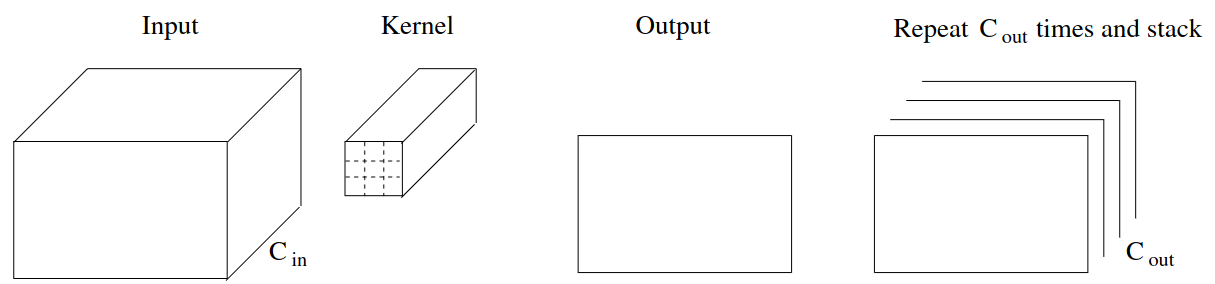
\includegraphics[width=0.65\linewidth]{./img/traditional_convolution.png}
            \caption{Example of traditional convolution}
        \end{figure}

        A single pass of a depth-wise separable convolution uses $C_\text{in}$ different $k \times k \times 1$ kernels first to obtain $C_\text{in}$ images.
        Then, a $1 \times 1 \times C_\text{in}$ kernel is used to obtain an output image of $1$ channel. 
        The last 1D kernel is repeated for a $C_\text{out}$ number of times (with different kernels).
        \begin{figure}[H]
            \centering
            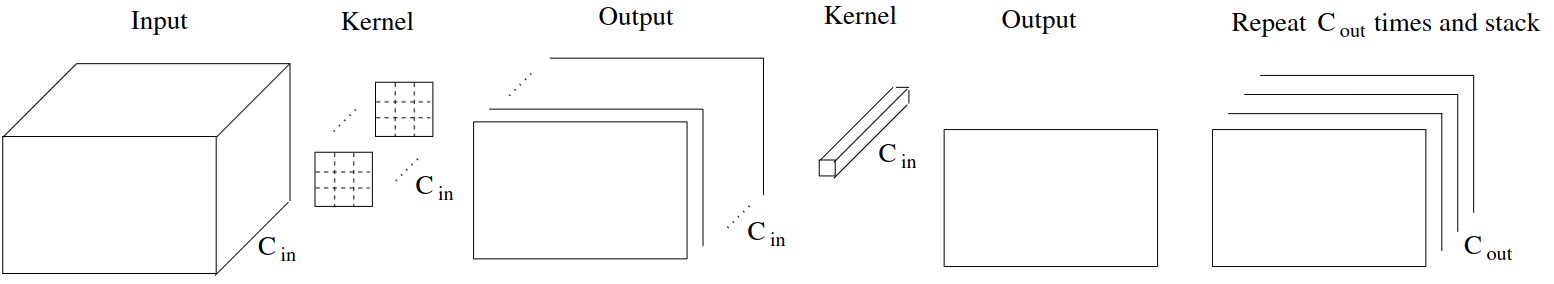
\includegraphics[width=0.85\linewidth]{./img/depthwise_separable_convolution.png}
            \caption{Example of depth-wise separable convolution}
        \end{figure}
\end{description}


\subsection{Parameters}

The number of parameters of a depth-wise separable convolutional layer is given by:
\[ (K_\text{w} \cdot K_\text{h}) \cdot D_\text{in} + (1 \cdot 1 \cdot D_\text{in}) \cdot D_\text{out} \]
where:
\begin{itemize}
    \item $K_\text{w}$ is the width of the kernel.
    \item $K_\text{h}$ is the height of the kernel.
    \item $D_\text{in}$ is the input depth.
    \item $D_\text{out}$ is the output depth.
\end{itemize}



\section{Residual learning}

\begin{description}
    \item[Residual connection] \marginnote{Residual connection}
        Sum the input of a layer to its output.
        \begin{figure}[H]
            \centering
            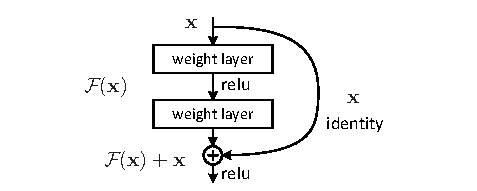
\includegraphics[width=0.5\linewidth]{./img/_residual_connection.pdf}
            \caption{Residual connection}
        \end{figure}

        \begin{remark}
            The sum operation can be substituted with the concatenation.
        \end{remark}

        \begin{remark}
            The effectiveness of residual connections is only shown empirically.
        \end{remark}

        \begin{remark}
            By adding the input, without passing through the activation function,
            might help to propagate the gradient from higher layers to lower layers
            and avoid the risk of vanishing gradient.
            
            Another interpretation is that, by learning the function $F(x) + x$, it is easier for the model to represent, if it needs to, the identity function as 
            the problem is reduced to learn $F(x) = 0$.
            On the other hand, without a residual connection, learning $F(x) = x$ from scratch might be harder.
        \end{remark}
\end{description}



\section{Transfer learning and fine-tuning}

\begin{description}
    \item[Transfer learning] \marginnote{Transfer learning}
        Reuse an existing model by appending some new layers to it.
        Only the new layers are trained.

    \item[Fine-tuning] \marginnote{Fine-tuning}
        Reuse an existing model by appending some new layers to it.
        The existing model (or part of it) is trained alongside the new layers.
\end{description}

\begin{remark}
    In computer vision, reusing an existing model makes sense as 
    the first convolutional layers tend to learn primitive concepts that are independent of the downstream task.
\end{remark}



\section{Other types of convolution}

\begin{description}
    \item[Transposed convolution / Deconvolution] \marginnote{Transposed convolution / Deconvolution}
        Convolution to upsample the input (i.e. each pixel is upsampled into a $k \times k$ patch).

        \begin{remark}
            A transposed convolution can be interpreted as a normal convolution with stride $< 1$.
        \end{remark}


    \item[Dilated convolution] \marginnote{Dilated convolution}
        Convolution computed using a kernel that does not consider contiguous pixels.

        \begin{figure}[H]
            \centering
            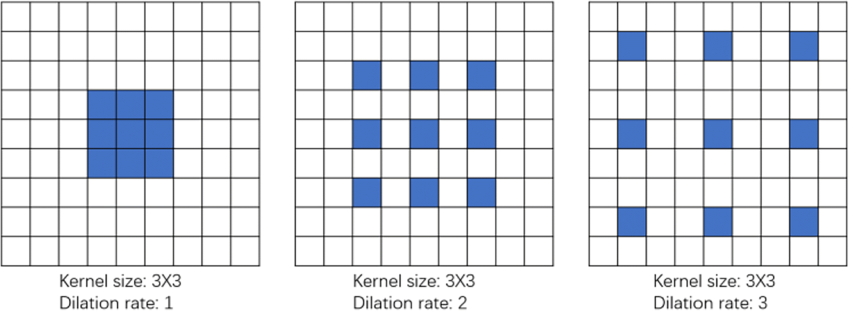
\includegraphics[width=0.5\linewidth]{./img/dilated_convolution.png}
            \caption{Examples of dilated convolutions}
        \end{figure}

        \begin{remark}
            Dilated convolutions allow the enlargement of the receptive field without an excessive number of parameters.
        \end{remark}

        \begin{remark}
            Dilated convolutions are useful in the first layers when processing high-resolution images (e.g. temporal convolutional networks).
        \end{remark}
\end{description}



\section{Normalization layer}

A normalization layer has the empirical effects of:
\begin{itemize}
    \item Stabilizing and possibly speeding up the training phase.
    \item Increasing the independence of each layer (i.e. maintain a similar magnitude of the weights at each layer).
\end{itemize}

\begin{description}
    \item[Batch normalization] \marginnote{Batch normalization}
        Given an input batch $X$, a batch normalization layer outputs the following:
        \[ \gamma \frac{X - \mu}{\sqrt{\sigma^2 + \varepsilon}} + \beta \]
        where:
        \begin{itemize}
            \item $\gamma$ and $\beta$ are learned parameters.
            \item $\varepsilon$ is a small constant.
            \item $\mu$ is the mean and $\sigma^2$ is the variance.
                Depending on when the layer is applied, these values change:
                \begin{descriptionlist}
                    \item[Training]
                        $\mu$ and $\sigma^2$ are computed from the input batch $X$.
        
                    \item[Inference] 
                        $\mu$ and $\sigma^2$ are computed from the training data. 
                        Usually, it is obtained as the moving average of the values computed from the batches during training.
                \end{descriptionlist}
        \end{itemize}
\end{description}



\section{Gradient ascent}


\subsection{Hidden layer visualization}
\marginnote{Hidden layer visualization}

Visualize what type of input features activate a neuron.

\begin{description}
    \item[Image ascent approach] 
        During training, the loss function of a neural network $\mathcal{L}(\vec{x}; \vec{\theta})$ is 
        parametrized on the weights $\vec{\theta}$ while the input $\vec{x}$ is fixed.
        
        To visualize the patterns that activate a (convolutional) neuron, it is possible to invert the optimization process
        by fixing the parameters $\vec{\theta}$ and optimizing an image $\vec{x}$ so that the loss function becomes $\mathcal{L}(\vec{\theta}; \vec{x})$.
        The process works as follows:
        \begin{enumerate}
            \item Start with a random image $\vec{x}$.
            \item Do a forward pass with $\vec{x}$ as input and keep track of the activation function $a_i(\vec{x})$ of the neuron(s) of interest.
            \item Do a backward pass to compute the gradient $\frac{\partial a_i(\vec{x})}{\partial \vec{x}_{i,j}}$ (i.e. chain rule) for each pixel $(i, j)$ of the image.
            \item Update the image as $\vec{x} = \vec{x} + \eta \frac{\partial a_i(\vec{x})}{\partial \vec{x}}$.
            \item Repeat until the activation function $a_i(\vec{x})$ is high enough.
        \end{enumerate}

        \begin{figure}[H]
            \centering
            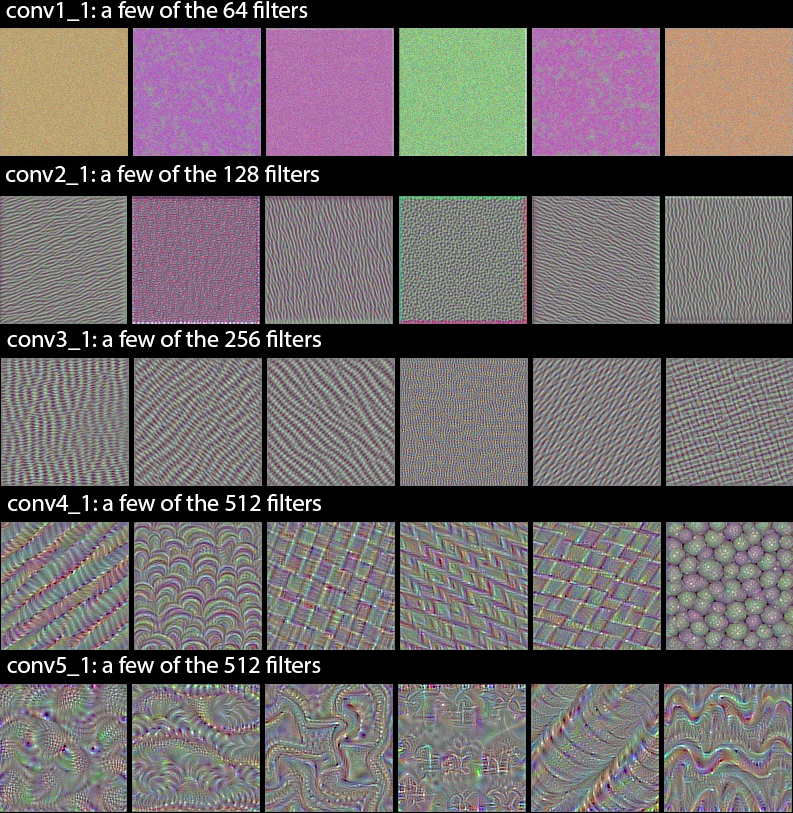
\includegraphics[width=0.5\linewidth]{./img/cnn_visualization_ascent.png}
            \caption{Example of generative image ascent visualization approach}
        \end{figure}

    \item[Generative approach]
        Starting from an image $\hat{\vec{x}}$ that makes a specific layer $l$ output $\Theta_l(\hat{\vec{x}})$, 
        generate another image $\vec{x}$ that makes the same layer $l$ output a similar value $\Theta_l(\vec{x}) \approx \Theta_l(\hat{\vec{x}})$
        (i.e. it cannot distinguish between $\vec{x}$ and $\hat{\vec{x}}$).

        Fixed $\hat{\vec{x}}$, the problem can be solved as an optimization problem:
        \[ \arg\min_{\vec{x}} \Big\{ l\big( \Theta_l(\vec{x}), \Theta_l(\hat{\vec{x}}) \big) + \lambda \mathcal{R}(\vec{x}) \Big\} \]
        where $l$ is a loss function to measure the distance between the two representations and 
        $\mathcal{R}$ is a regularizer.

        \begin{figure}[H]
            \centering
            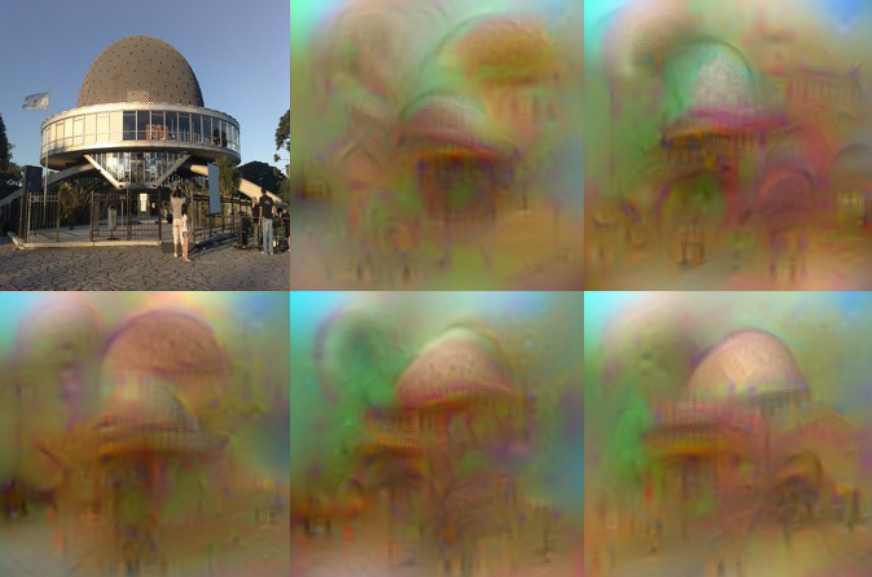
\includegraphics[width=0.6\linewidth]{./img/cnn_visualization_generative.png}
            \caption{Example of generative visualization approach}
        \end{figure}
\end{description}


\subsection{Inceptionism}
\marginnote{Inceptionism}

Employ the same techniques for hidden layer visualization to create psychedelic and abstract images.

\begin{description}
    \item[Deep dream] \marginnote{Deep dream}
        Iteratively apply gradient ascent on an image:
        \begin{enumerate}
            \item Train a neural network for image classification.
            \item Repeatedly modify an input image using gradient ascent to improve the activation of a specific neuron.
        \end{enumerate}

        After enough iterations, the features that the target neuron learned to recognize during training are injected into the input image,
        even if that image does not have that specific feature.

        \begin{remark}
            Strong regularizers are used to prioritize features that statistically resemble real images.
        \end{remark}

    \item[Content enhancing] \marginnote{Content enhancing}
        Same as above, but instead of selecting a neuron, an entire layer is fixed and the input image is injected with whatever that layer detects.

    \begin{figure}[H]
        \centering
        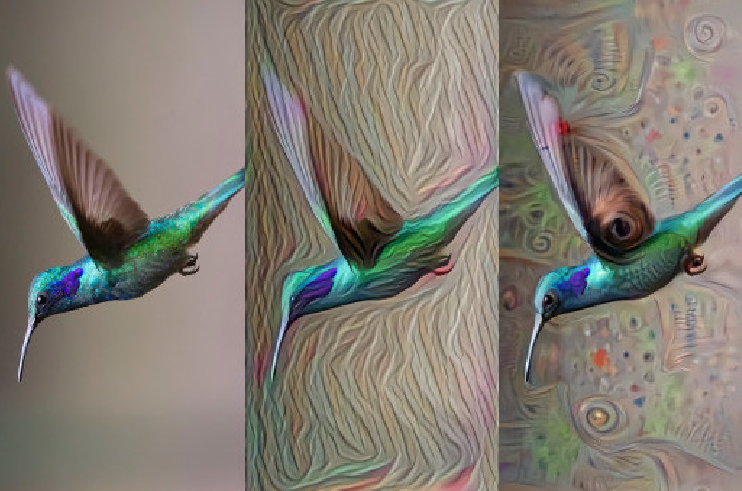
\includegraphics[width=0.55\linewidth]{./img/inceptionism.png}
        \caption{Example of deep dream images}
    \end{figure}
\end{description}


\subsection{Style transfer}
\marginnote{Style transfer}

Mimic the style of an image and transfer it to the content of another one.

\begin{description}
    \item[Internal representation approach] 
        Given a convolutional neural network pretrained for classification, the method can be divided into two parts:
        \begin{descriptionlist}
            \item[Content reconstruction] 
                Given an image $\hat{\vec{x}}$, consider the output of the $l$-th layer of the network.
                Its internal representation of the image has $C^l$ distinct channels (depending on the number of kernels)
                each with $M^l = W^l \cdot H^l$ elements (when flattened).
        
                The representation (feature map) of the $l$-th layer can therefore be denoted as $F^l \in \mathbb{R}^{C^l \times M^l}$
                and $F^l_{c, k}$ is used to denote the activation of the $c$-th filter applied at position $k$ of the $l$-th layer.
        
                As higher layers of a CNN capture high-level features, one of the high layers is selected and its feature map is used as the content representation.
        
                Given a content representation $\mathcal{C} = \hat{F}^l$ of $\hat{\vec{x}}$, chosen as the feature map at the $l$-th layer, 
                it is possible to reconstruct the original image $\hat{\vec{x}}$ starting from a random one $\vec{x}$ by minimizing the loss:
                \[ \mathcal{L}_\text{content}(\hat{\vec{x}}, \vec{x}, l) = \sum_{c, i} (F^l_{c, i} - \mathcal{C}_{c, i})^2 \]
                where $F^l$ is the feature representation of the random image $\vec{x}$.
        
            \item[Style reconstruction] 
                Given an image $\hat{\vec{y}}$ and its feature maps $F^l$ for $l \in \{1, \dots L\}$,
                at each layer $l$, the Gram matrix $G^l \in \mathbb{R}^{C^l \times C^l}$ obtained as the dot product between pairs of channels 
                (i.e. correlation between features extracted by different kernels):
                \[ G^l_{c_1, c_2} = F^l_{c_1} \odot F^l_{c_2} = \sum_{k} (F^l_{c_1, k} \cdot F^l_{c_2, k}) \]
                allows to capture the concept of style.
        
                The Gram matrices at each layer are considered as the style representation.
        
                Given the style representation $\mathcal{S}^1, \dots, \mathcal{S}^L$ of $\hat{\vec{y}}$,
                it is possible to reconstruct the same style of the original image $\hat{\vec{y}}$ starting from a random image $\vec{y}$ by minimizing the loss:
                \[ \mathcal{L}_\text{style}(\hat{\vec{y}}, \vec{y}) = \sum_{l=1}^{L} \gamma_l \left(\sum_{i,j} (G^l_{i, j} - \mathcal{S}^l_{i,j})^2 \right) \]
                where $\gamma_l$ is a weight assigned to each layer and $G^l$ is the $l$-th Gram matrix of the random image $\vec{y}$.
        \end{descriptionlist}
        
        Put together, given:
        \begin{itemize}
            \item An image $\hat{\vec{x}}$ from which the content has to be copied.
            \item An image $\hat{\vec{y}}$ from which the style has to be copied.
            \item The content representation $\mathcal{C}$ of $\hat{\vec{x}}$.
            \item The style representation $\mathcal{S}^1, \dots, \mathcal{S}^L$ of $\hat{\vec{y}}$.
        \end{itemize}
        A new random image $\vec{o}$ is fitted by minimizing the loss:
        \[ \mathcal{L}_\text{total} = \alpha \mathcal{L}_\text{content}(\hat{\vec{x}}, \vec{o}, l) + \beta \mathcal{L}_\text{style}(\hat{\vec{y}}, \vec{o}) \]
        where $\alpha$ and $\beta$ are hyperparameters.
        
        \begin{figure}[H]
            \centering
            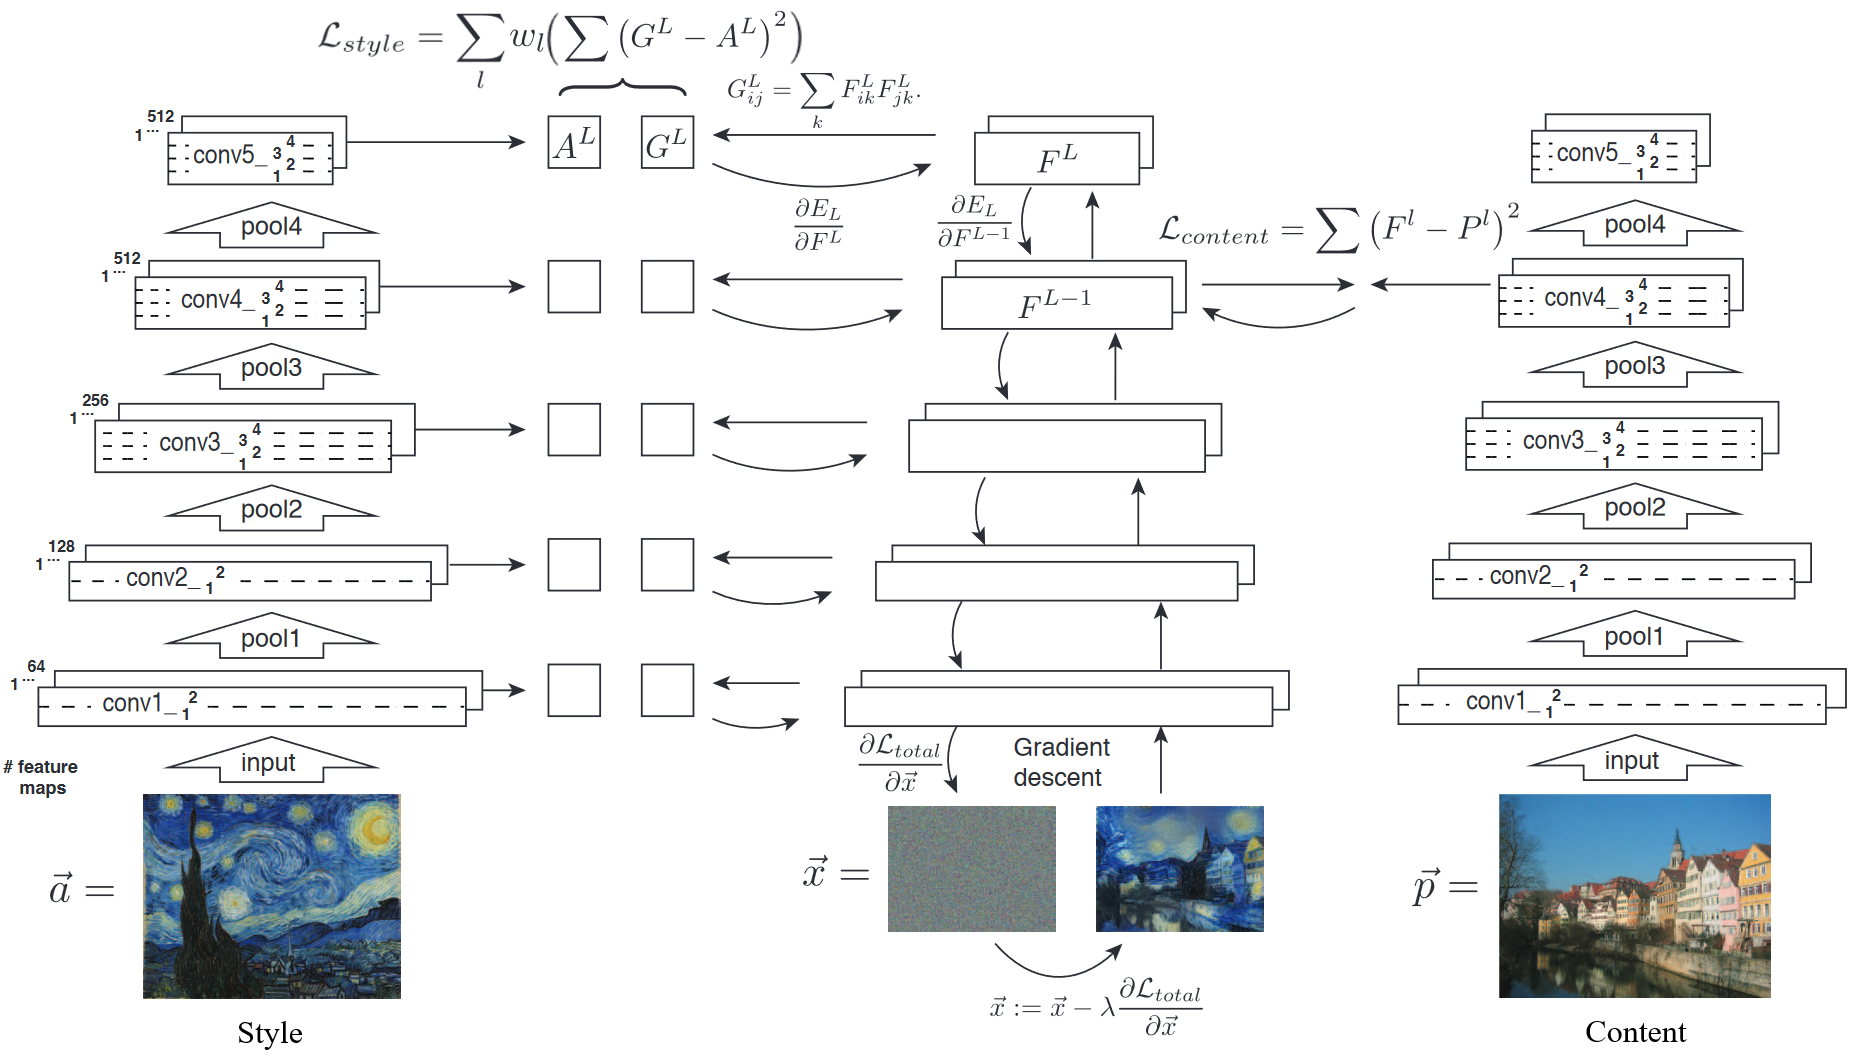
\includegraphics[width=0.95\linewidth]{./img/style_transfer.png}
            \caption{Internal representation style transfer workflow}
        \end{figure}

    \item[Perceptual loss approach]
        A CNN pretrained for classification is used as a loss network to compute perceptual loss functions
        to measure the difference in style and content between images.
        The representation for style and content is extracted in a similar way as above.

        The loss network is then kept fixed and an image transformation network is trained to transform its input $\vec{x}$ 
        into an image $\vec{y}$ compliant (i.e. minimizes the perceptual losses) with a given style image $\vec{y}_s$ and a content image $\vec{y}_c$ 
        (if the goal is to keep the content of the input, then $\vec{y}_c = \vec{x}$).

        \begin{figure}[H]
            \centering
            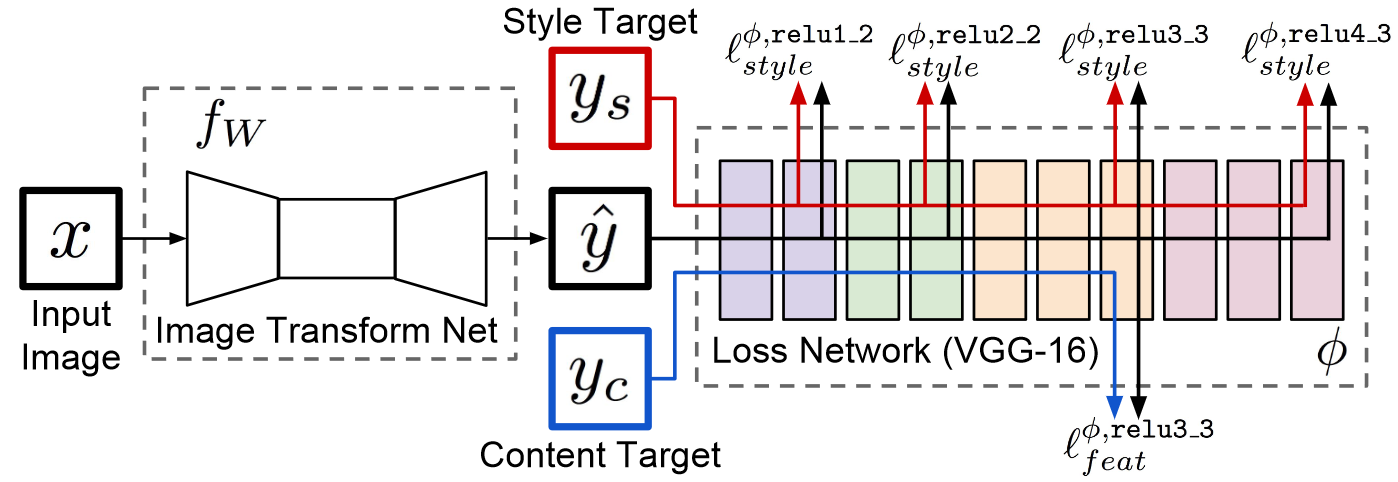
\includegraphics[width=0.55\linewidth]{./img/style_transfer_perceptual_loss.png}
            \caption{Perceptual loss style transfer workflow}
        \end{figure}
\end{description}



\section{Data manifold}


\subsection{Adversarial attacks}
\marginnote{Adversarial attacks}

Hijack a neural network classifier to forcefully predict a given class.

\begin{description}
    \item[Gradient ascent approach]
        White-box technique that uses gradient ascent to compute an image that the network classifies with the wanted class.

        Let:
        \begin{itemize}
            \item $\vec{x}$ be the input image.
            \item $f(\vec{x})$ the probability distribution that the network outputs.
            \item $c$ the wanted class.
            \item $p$ the wanted probability distribution (i.e. $p_c = 1$ and $p_i = 0$ elsewhere).
            \item $\mathcal{L}$ the loss function.
        \end{itemize}

        By iteratively updating the input image with the gradient of the loss function $\frac{\partial\mathcal{L}(f(\vec{x}), p)}{\partial\vec{x}}$ 
        computed wrt to $\vec{x}$,
        after enough iterations, the classifier will classify the updated $\vec{x}$ as $c$.

        \begin{remark}
            The updates computed from the gradient of the loss function are usually imperceptible.
        \end{remark}

        \begin{figure}[H]
            \centering
            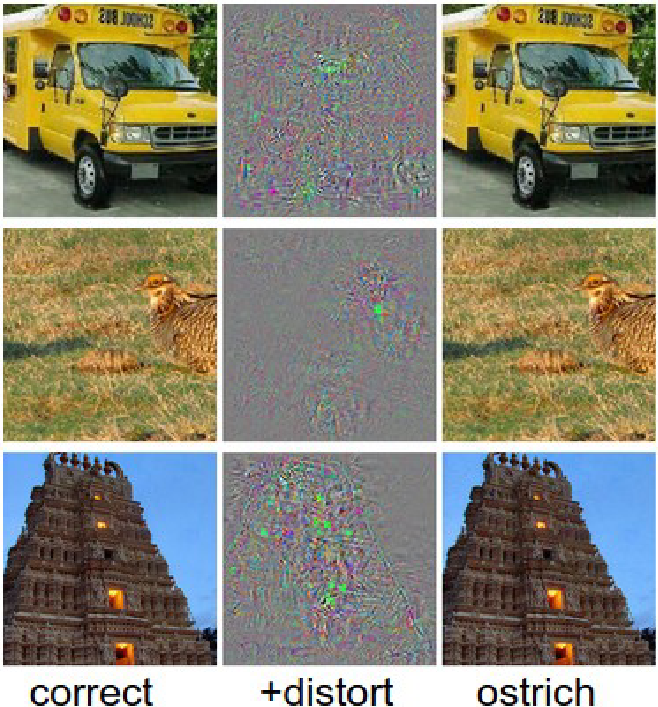
\includegraphics[width=0.25\linewidth]{./img/fooling_nn.png}
            \caption{Examples of hijacked classifications}
        \end{figure}

    \item[Evolutionary approach]
        Black-box technique based on an evolutionary approach.

        \begin{figure}[H]
            \centering
            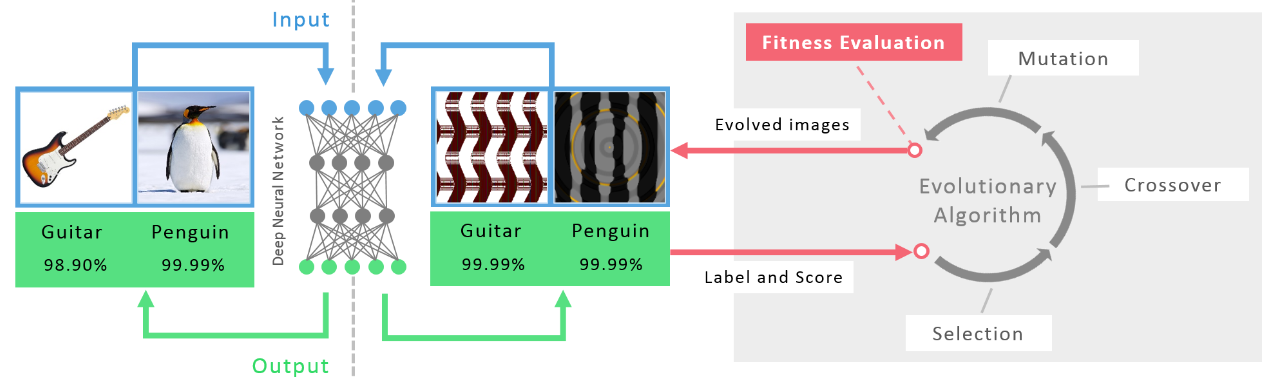
\includegraphics[width=0.8\linewidth]{./img/fooling_evolutionary.png}
            \caption{Workflow for evolutionary-based attacks}
        \end{figure}
\end{description}


\subsection{Manifold}

\begin{description}
    \item[Manifold] \marginnote{Manifold}
        Area of the feature space that represents "natural" images (i.e. images with a meaning an without artificial noise).

        This area is usually organized along a smooth surface which is a minimal portion of the entire space of all the possible images.

        \begin{figure}[H]
            \centering
            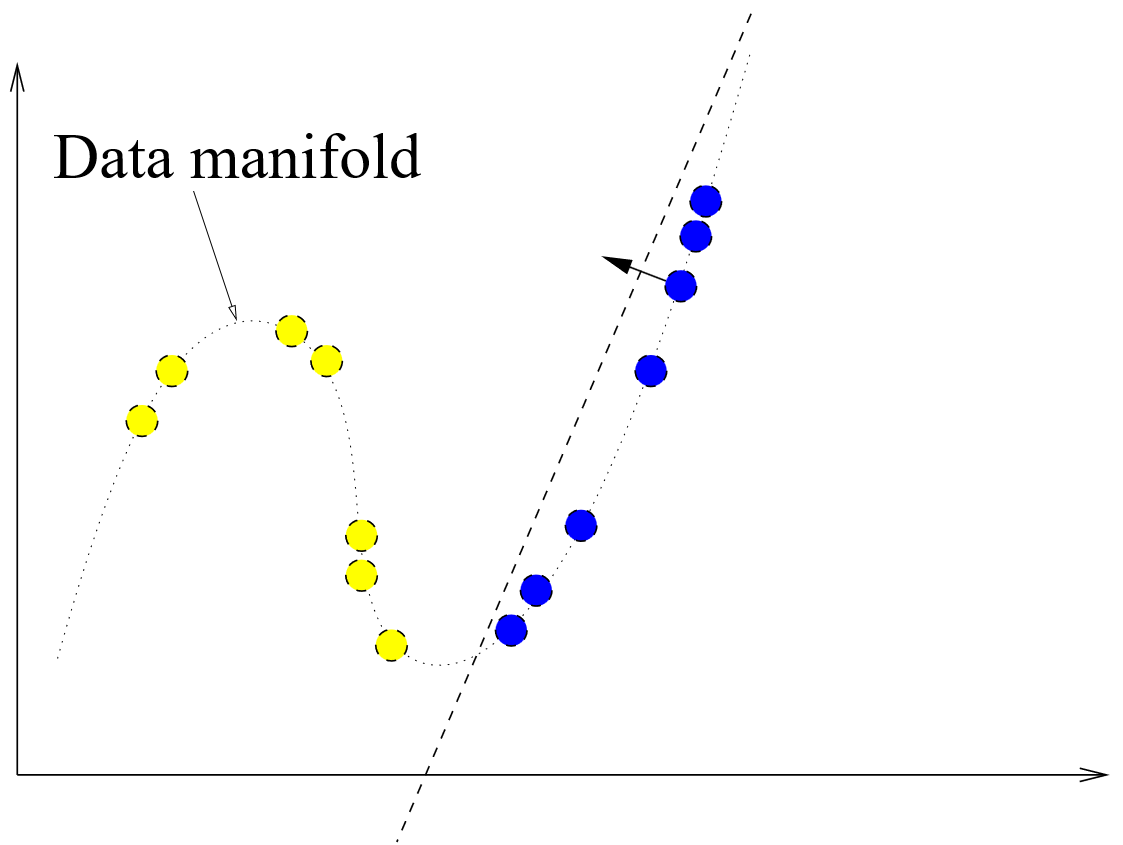
\includegraphics[width=0.35\linewidth]{./img/manifold.png}
            \caption{Example of manifold in two dimensions}
        \end{figure}
\end{description}

\begin{remark}
    As one cannot know where the classifier draws the boundaries,
    a tiny change in the data might cause a misclassification.

    Adversarial attacks also exploit this to cause misclassifications.
\end{remark}

\begin{remark}
    Inceptionism aims to modify the data while remaining in the manifold.
\end{remark}


\subsection{Autoencoders}
\marginnote{Autoencoder}

Network composed of two components:
\begin{descriptionlist}
    \item[Encoder]
        Projects the input into an internal representation of lower dimensionality.

    \item[Decoder]
        Reconstructs the input from its internal representation.
\end{descriptionlist}

\begin{figure}[H]
    \centering
    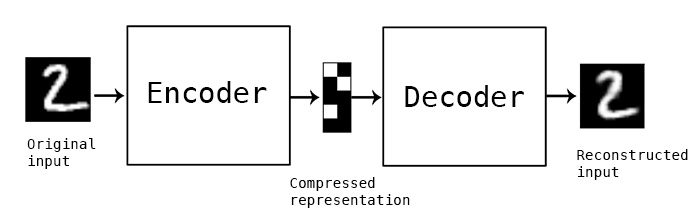
\includegraphics[width=0.5\linewidth]{./img/autoencoder.png}
    \caption{Autoencoder structure}
\end{figure}

An autoencoder has the following properties:
\begin{descriptionlist}
    \item[Data-specific] It only works on data with a strong correlation (i.e. with regularities in the feature space).
    \item[Lossy] By passing through the internal representation, the reconstruction of the input is nearly always degraded.
    \item[Self-supervised] Training happens directly on unlabelled data.
\end{descriptionlist}

Applications of autoencoders are:
\begin{descriptionlist}
    \item[Denoising] 
        Train the autoencoder to reconstruct noiseless data.
        Given an image, the input is a noisy version of it, while the output is expected to be similar to the original image.

    \item[Anomaly detection]
        As autoencoders are data-specific, they will perform poorly on data different from those used for training.

        This allows to detect anomalies by comparing the quality of the reconstruction.
        If the input is substantially different from the training data (or has been attacked with an artificial manipulation),
        the reconstructed output is expected to have poor quality.

        \begin{figure}[H]
            \centering
            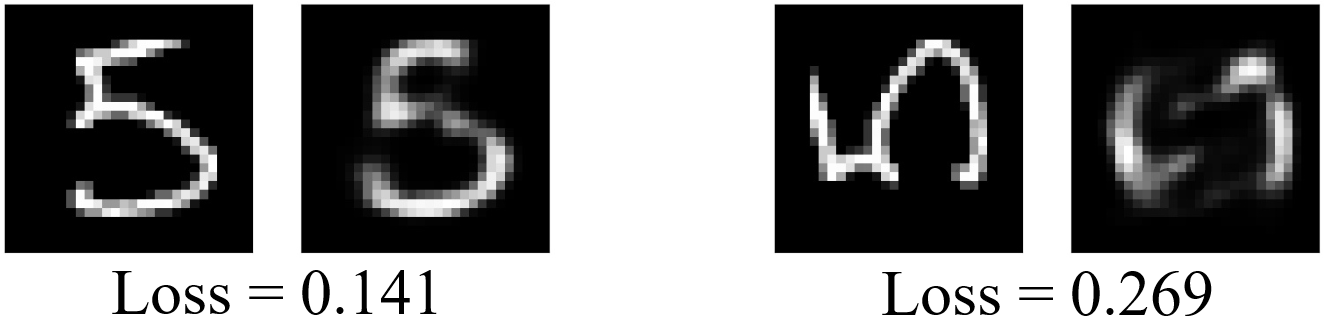
\includegraphics[width=0.5\linewidth]{./img/autoencoder_anomaly.png}
            \caption{Example of anomaly detection}
        \end{figure}
\end{descriptionlist}



\section{Segmentation}

\begin{description}
    \item[Semantic segmentation] \marginnote{Semantic segmentation}
        Classify the pixels of an image depending on the category it belongs to.

        \begin{remark}
            Creating a dataset for segmentation is expensive.
        \end{remark}
\end{description}

\begin{figure}[H]
    \centering
    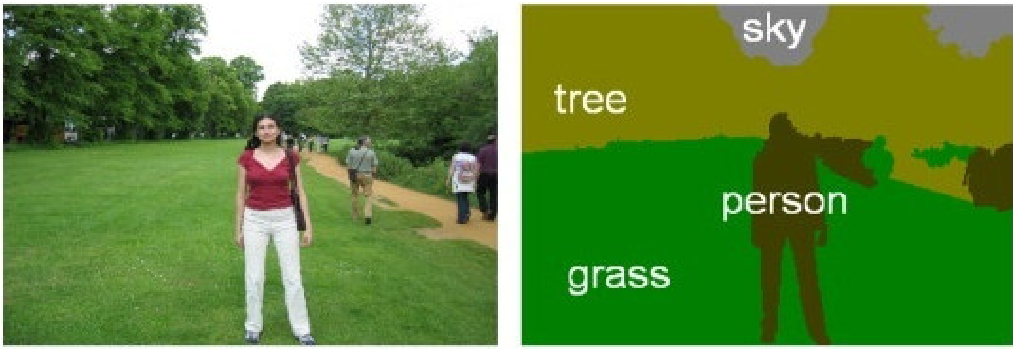
\includegraphics[width=0.75\linewidth]{./img/semantic_segmentation.png}
    \caption{Example of semantic segmentation}
\end{figure}


\subsection{Convolutionalization}
\marginnote{Convolutionalization}

Given a pre-trained image classification network,
it can be adapted into a segmentation network by converting its final dense layers into convolutions
with kernel size $1 \times 1$ and depth equal to the number of neurons in that layer.

\begin{figure}[H]
    \centering
    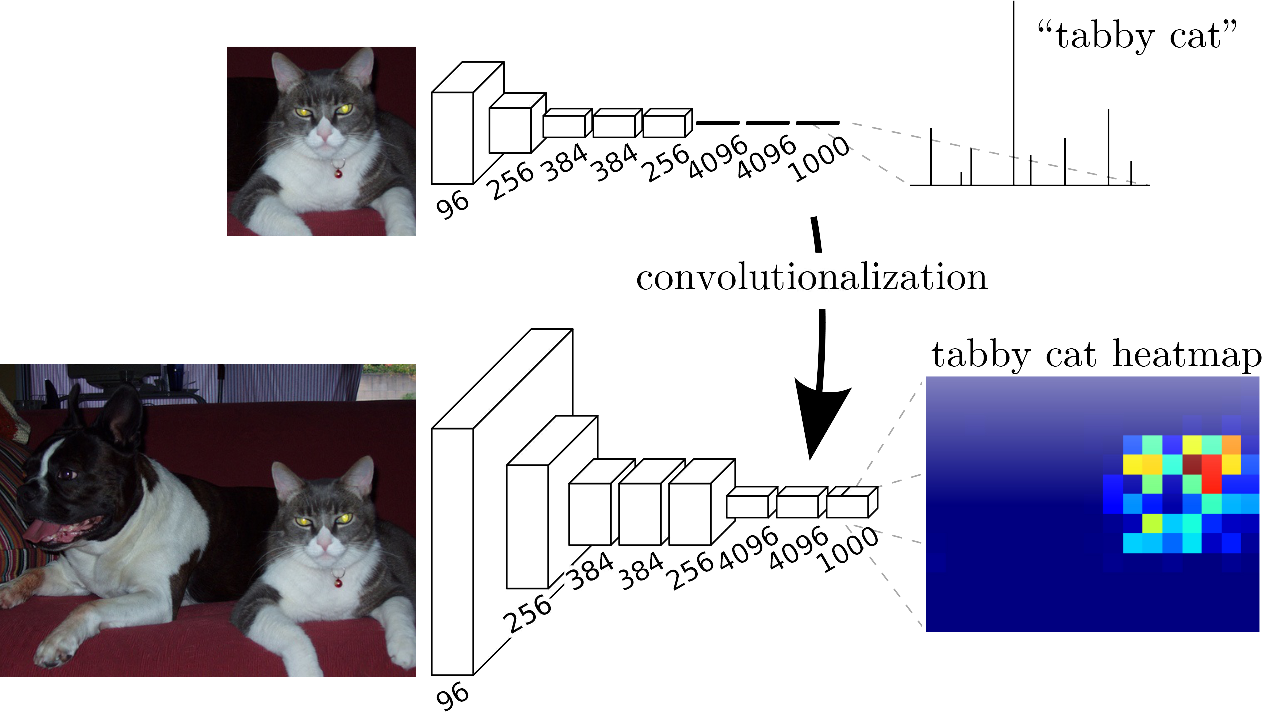
\includegraphics[width=0.5\linewidth]{./img/_convolutionalization.pdf}
    \caption{Example of convolutionalization}
\end{figure}

The resulting model has the following behavior:
\begin{itemize}
    \item It takes as input an image of arbitrary shape. This is possible as the network is composed of only convolutions (i.e. it can be seen as a single big convolution).
    \item It outputs a heatmap of activations of the different object classes (i.e. the categories of the pre-trained classification network).
\end{itemize}

As the output is obtained through a series of convolutions, its shape does not match the input image.
Therefore, the initial output heatmap needs to be upsampled by using transposed convolutions.

To avoid losing information from previous layers, the original work proposes to use skip connections before upsampling.

\begin{figure}[H]
    \centering
    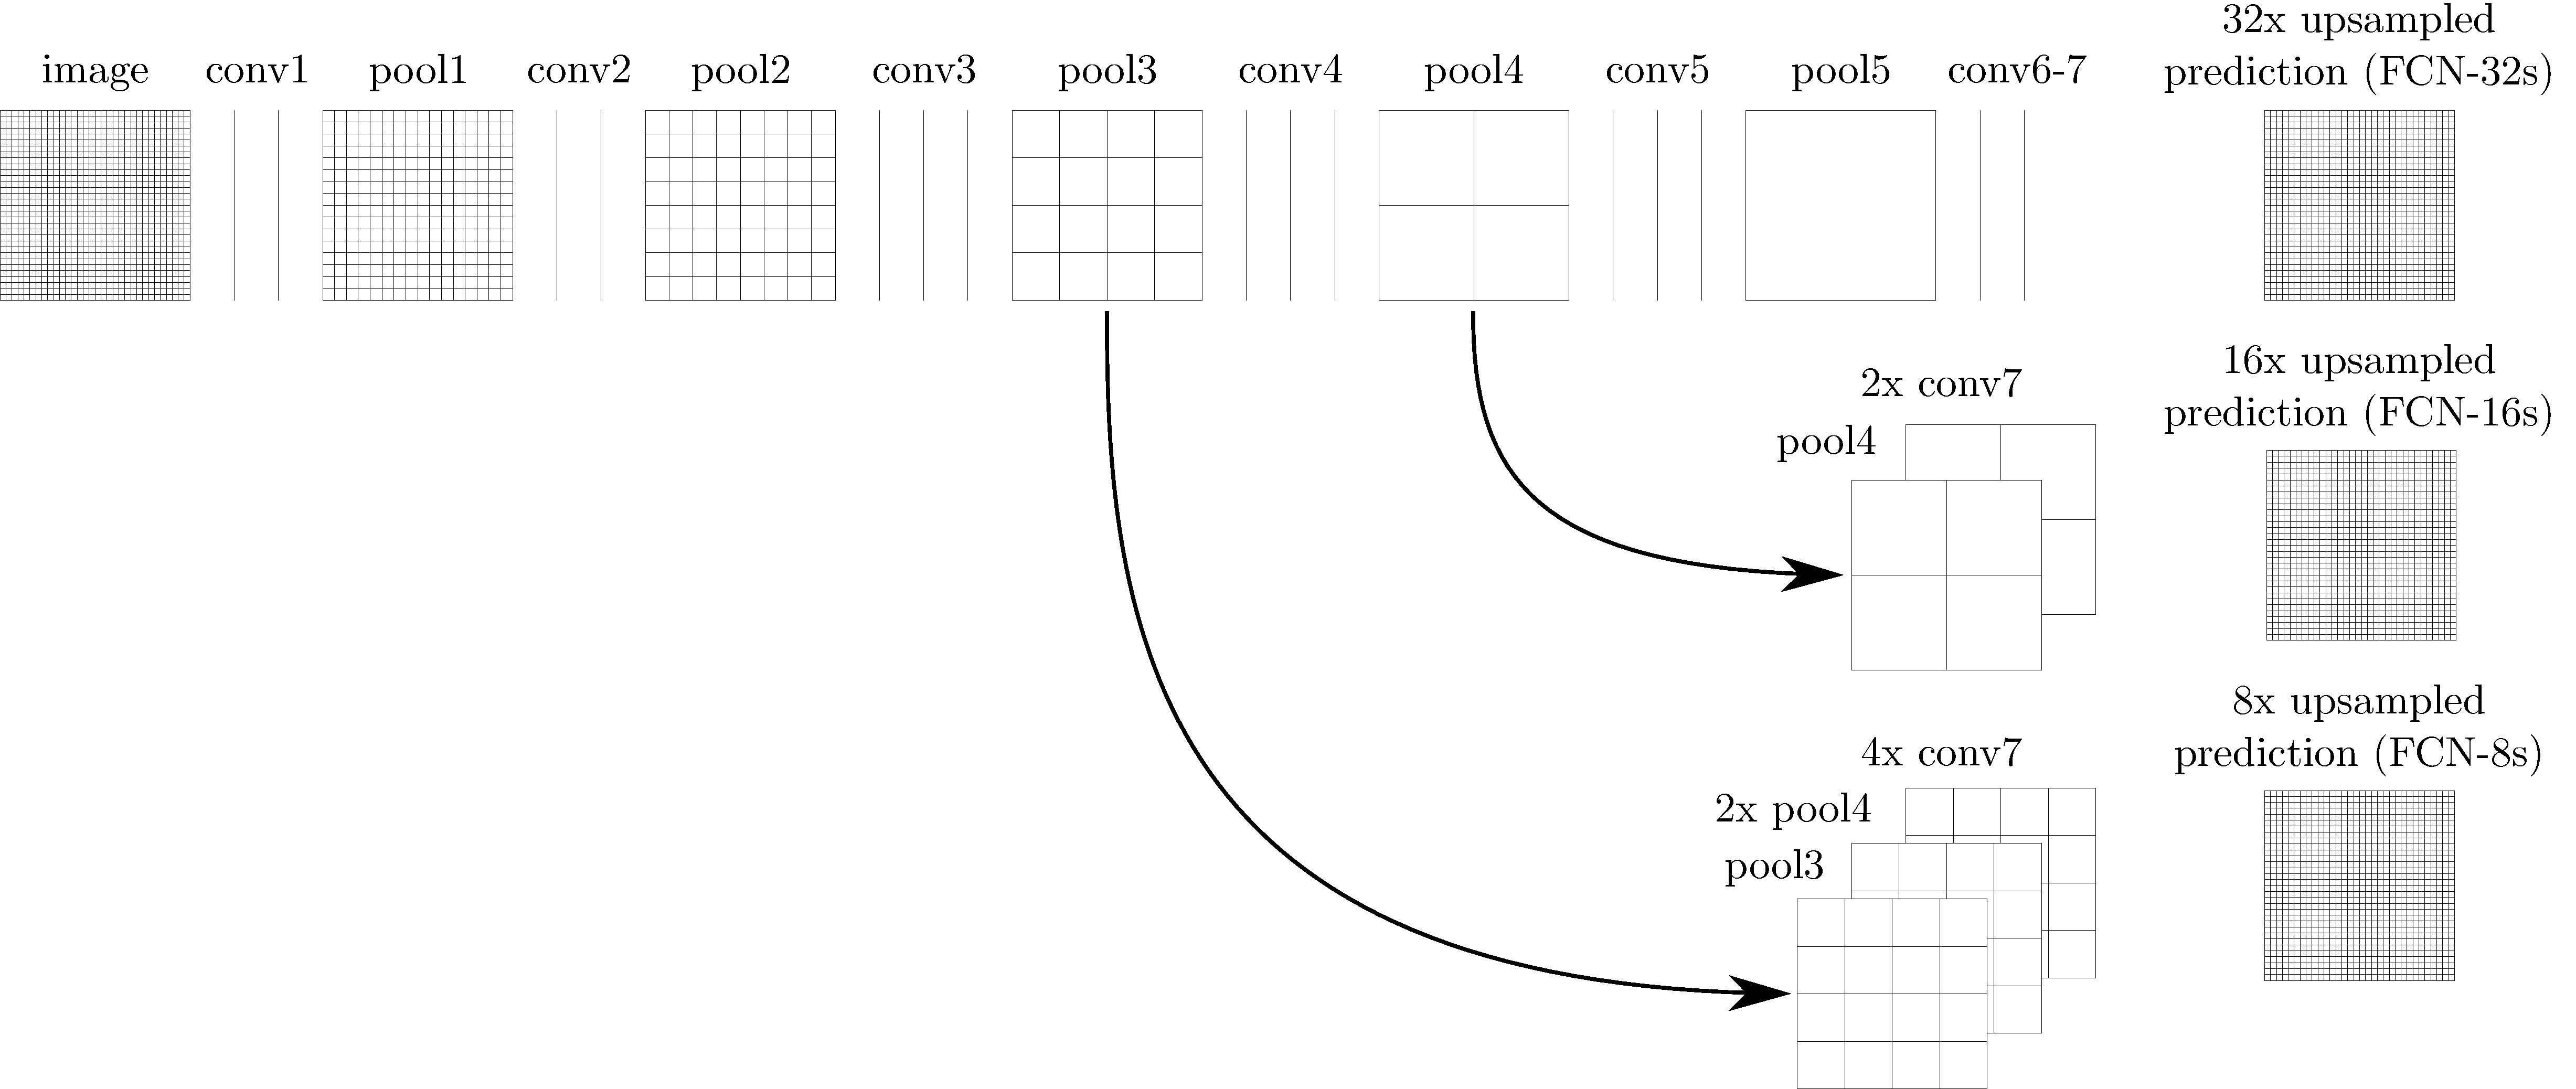
\includegraphics[width=0.95\linewidth]{./img/_convolutionalization_skip.pdf}
    \caption{
        Examples of upsampling.
        The first row shows the upsampling process of the output (\texttt{conv7}) without skip connections.
        The second row shows the upsampling process with a skip connection from the second last pooling layer (\texttt{pool4}):
        the output (\texttt{conv7}) is partially upsampled to match the shape of the skip connectionm, then upsampling is done on their concatenation.
        The third row shows the upsampling process with skip connections up to the third last pooling layer (\texttt{pool3}).
    }
\end{figure}


\subsection{U-net}
\marginnote{U-net}

Segmentation architecture that does not rely on a pre-trained classification network.

The architecture is composed of two steps:
\begin{descriptionlist}
    \item[Downsampling] Using convolutions and max-pooling.
    \item[Upsampling] Using transposed convolutions and skip connections.
\end{descriptionlist}

\begin{remark}
    An interpretation of the two operations is the following:
    \begin{descriptionlist}
        \item[Downsampling] Aims to find what the image contains.
        \item[Upsampling] Aims to find where the found objects are.
    \end{descriptionlist}
\end{remark}

\begin{figure}[H]
    \centering
    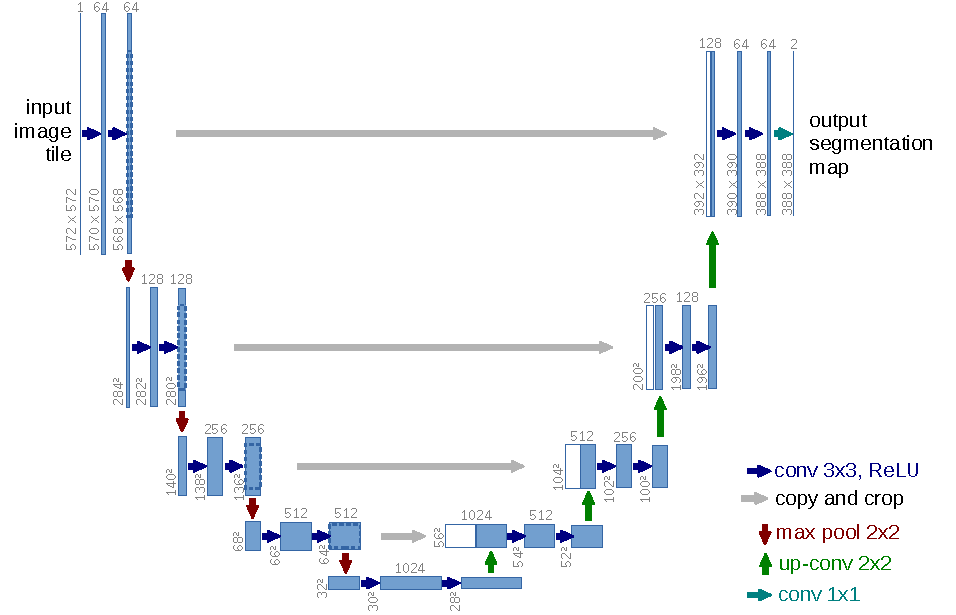
\includegraphics[width=0.75\linewidth]{./img/_unet.pdf}
    \caption{Example of U-net architecture without padding}
\end{figure}

\begin{remark}
    In the original work, the architecture is defined using cropping and without padding, making the output shape smaller than the input.
    Segmentation was therefore done on a cropped portion of the input image.

    Another approach is to use padding to maintain the same shape of the input in the output.
\end{remark}



\section{Object detection}

\begin{description}
    \item[Intersection over union] \marginnote{Intersection over union}
        Metric used to determine the quality of a bounding box w.r.t. a ground truth:
        \[ \texttt{IoU}(A, B) = \frac{\vert A \cap B \vert}{\vert A \cup B \vert} \]

    \item[Object detection] \marginnote{Object detection}
        Find bounding boxes containing a specific object or category.

        There are two main strategies:
        \begin{description}
            \item[Region proposal] \marginnote{Region proposal}
                Object-independent method that uses selective search algorithms to exploit the texture and the structure of the image to find locations of interest.

            \item[Single-shot] \marginnote{Single shot}
                Fast method oriented towards real-time applications.
        \end{description}

        \begin{figure}[H]
            \centering
            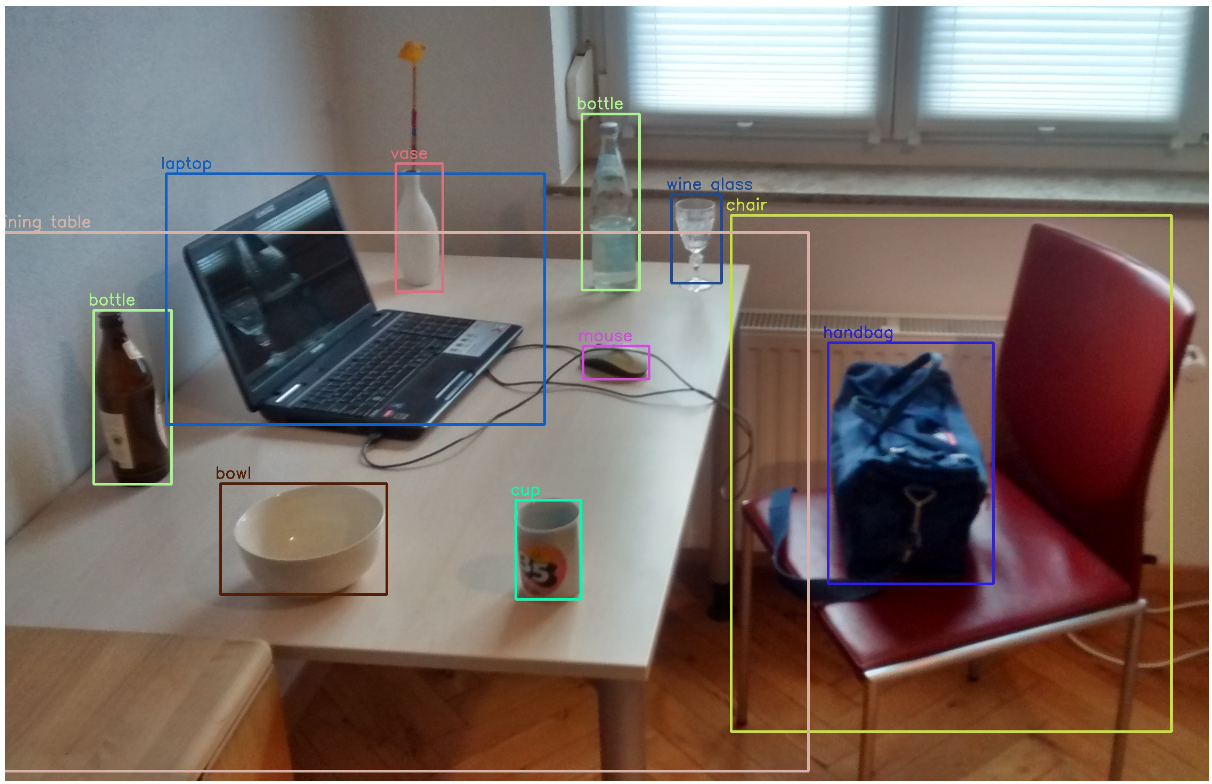
\includegraphics[width=0.35\linewidth]{./img/object_detection.png}
            \caption{Example of bounding boxes}
        \end{figure}
\end{description}


\subsection{YOLOv3}

YOLO is a fully convolutional neural network belonging to the family of single-shot methods.
% Given an image, YOLO downsamples it to obtain a feature map .
% Each cell of the feature map makes bounding box predictions.

\begin{description}
    \item[Anchor box] \marginnote{Anchor box}
        It has been shown that directly predicting the width and height of the bounding boxes leads to unstable gradients during training.
        A common solution to this problem is to use pre-defined bounding boxes (anchors).

        Anchors are selected using k-means clustering on the bounding boxes of the training set using \texttt{IoU} as metric (i.e. the most common shapes are identified).
        Then, the network learns to draw bounding boxes by placing and scaling the anchors.


    \item[Architecture] \marginnote{YOLO architecture}
        An input image is progressively downsampled through convolutions by a factor of $2^5$ to obtain a feature map of $S \times S$ cells
        (e.g. a $416 \times 416$ image is downsampled into a $13 \times 13$ grid).

        Each entry of the feature map has a depth of $(B \times (5+C))$ where:
        \begin{itemize}
            \item $B$ is the number of bounding boxes (one per anchor) the cell proposes.
            \item $C$ is the number of object classes.
        \end{itemize}

        Therefore, each bounding box prediction has associated $5+C$ attributes:
        \begin{itemize}
            \item $t_x$ and $t_y$ describe the center coordinates of the box (relative to the predicting cell).
            \item $t_w$ and $t_h$ describe the width and height of the box (relative to the anchor).
            \item $p_o$ is an objectness score that indicates the probability that an object is contained in the predicted bounding box (useful for thresholding).
            \item $p_1, \dots, p_C$ are the probabilities associated to each class. 
                Since YOLOv3, the probability of each class is given by a sigmoid instead of passing everything through a softmax.
                This allows to associate an object with multiple categories.
        \end{itemize}
        
        \begin{figure}[H]
            \centering
            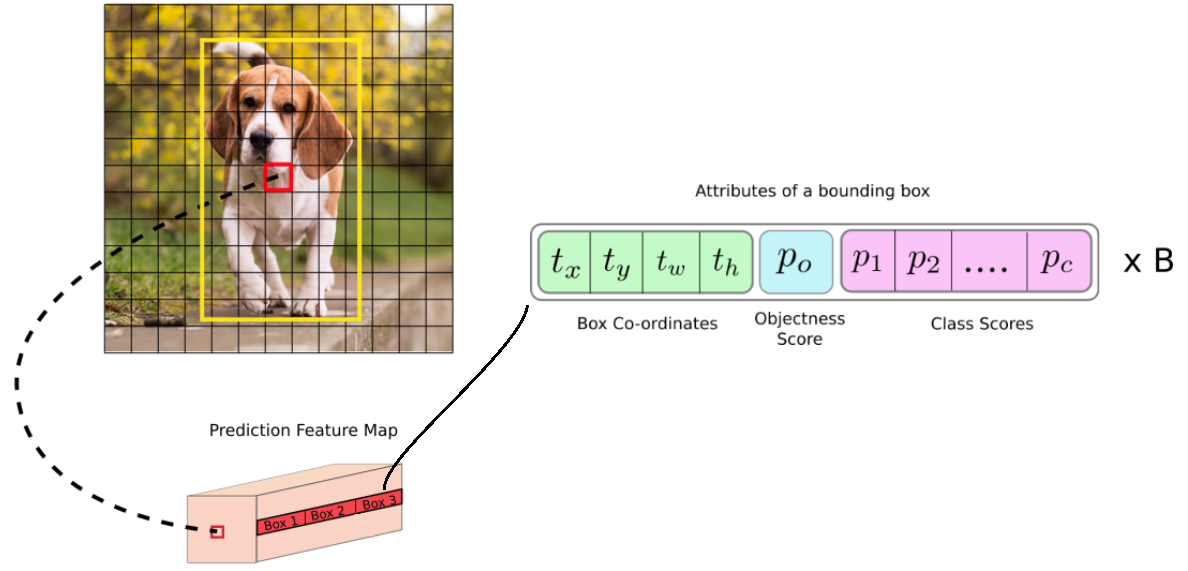
\includegraphics[width=0.6\linewidth]{./img/yolo_architecture.png}
        \end{figure}


    \item[Inference] \marginnote{YOLO inference}
        \begin{remark}
            Each cell of the feature map is identified by a set of coordinates relative to the feature map itself 
            (e.g. the first cell is at coordinate $(0,0)$, the one to its right is at $(0, 1)$).    
        \end{remark}

        Given a cell of the feature map at coordinates $(c_x, c_y)$, consider its $i$-th bounding box prediction.
        The bounding box is computed using the following parameters:
        \begin{itemize}
            \item The predicted relative position and dimension $\langle t_x, t_y, t_w, t_h \rangle$ of the box.
            \item The width $p_w$ and height $p_h$ of the anchor associated with the $i$-th prediction of the cell.
        \end{itemize}
        Then, the bounding box position and dimension (relative to the feature map) are computed as follows:
        \[
            \begin{split}
                b_x &= c_x + \sigma(t_x) \\
                b_y &= c_y + \sigma(t_y) \\
                b_w &= p_w \cdot e^{t_w} \\
                b_h &= p_h \cdot e^{t_h} \\
            \end{split}  
        \]
        where:
        \begin{itemize}
            \item $(b_x, b_y)$ are the coordinates of the center of the box.
            \item $b_w$ and $b_h$ are the width and height of the box.
            \item $\sigma$ is the sigmoid function.
        \end{itemize}

        \begin{figure}[H]
            \centering
            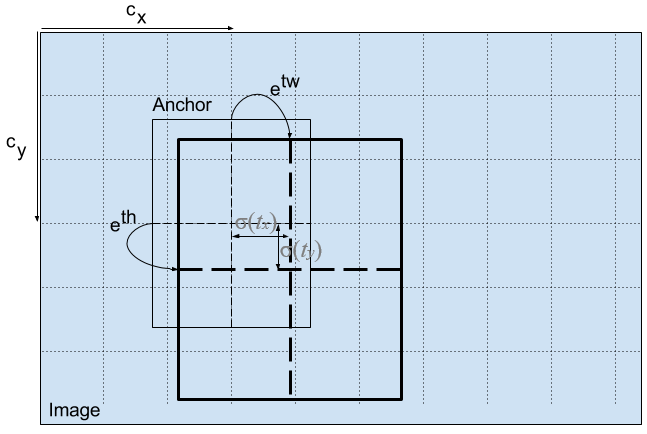
\includegraphics[width=0.5\linewidth]{./img/yolo_anchor.png}
        \end{figure}


    \item[Training] \marginnote{YOLO training}
        During training, for each ground truth bounding box, 
        only the cell at its center and the anchor with the highest \texttt{IoU} are considered for its prediction.
        In other words, only that combination of cell and anchor influences the loss function.

        Given a $S \times S$ feature map and $B$ anchors, for each prediction, YOLO uses two losses:
        \begin{descriptionlist}
            \item[Localization loss] 
                Measures the positioning of the bounding boxes:
                \[ 
                    \mathcal{L}_\text{loc} = \lambda_\text{coord} \sum_{i=0}^{S \times S} \sum_{j=0}^{B} \mathbbm{1}_{ij}^\text{obj} \Big( 
                        (x_i - \hat{x}_i)^2 + (y_i - \hat{y}_i)^2 +
                        (\sqrt{w_i} - \sqrt{\hat{w}_i})^2 + (\sqrt{h_i} - \sqrt{\hat{h}_i})^2
                    \Big) 
                \]
                where:
                \begin{itemize}
                    \item $\mathbbm{1}_{ij}^\text{obj}$ is a delta function that is 1 if the $j$-th anchor of the $i$-th cell is responsible for detecting the object.
                    \item $(x_i, y_i)$ are the predicted coordinates of the box. $(\hat{x}_i, \hat{y}_i)$ are the ground truth coordinates.
                    \item $w_i$ and $h_i$ are the predicted width and height of the box. $\hat{w}_i$ and $\hat{h}_i$ are the ground truth dimensions.
                    \item $\lambda_\text{coord}$ is a hyperparameter (the default is 5).
                \end{itemize}

            \item[Classification loss] 
                Considers the objectness score and the predicted classes:
                \[
                    \begin{split}
                        \mathcal{L}_\text{cls} = &\sum_{i=0}^{S \times S} \sum_{j=0}^{B} (\mathbbm{1}_{ij}^\text{obj} + \lambda_\text{no-obj}(1-\mathbbm{1}_{ij}^\text{obj}))(C_{ij} - \hat{C}_{ij})^2 \\
                            &+ \sum_{i=0}^{S \times S} \sum_{c \in \mathcal{C}} \mathbbm{1}_{i}^\text{obj} (p_i(c) - \hat{p}_i(c))^2
                    \end{split}
                \]
                where:
                \begin{itemize}
                    \item $\mathbbm{1}_{ij}^\text{obj}$ is defined as above.
                    \item $\mathbbm{1}_{i}^\text{obj}$ is 1 if the $i$-th cell is responsible for classifying the object.
                    \item $C_{ij}$ is the predicted objectness score. $\hat{C}_{ij}$ is the ground truth.
                    \item $p_i(c)$ is the predicted probability of belonging to class $c$. $\hat{p}_i(c)$ is the ground truth.
                    \item $\lambda_\text{no-obj}$ is a hyperparameter (the default is 0.5). 
                        It is useful to down-weight cells that are not responsible for detecting this specific instance.
                \end{itemize}
        \end{descriptionlist}

        The final loss is the sum of the two losses:
        \[\mathcal{L} = \mathcal{L}_\text{loc} + \mathcal{L}_\text{cls} \]
\end{description}


\subsection{Multi-scale processing}

\begin{description}
    \item[Feature pyramid] \marginnote{Feature pyramid}
        Techniques to manipulate the input image to detect objects at different scales.

        Possible approaches are:
        \begin{descriptionlist}
            \item[Featurized image pyramid] 
                A pyramid of images at different scales is built. The features at each scale are computed independently (which makes this approach slow).

            \item[Single feature map] 
                Progressively extract features from a single image and only use features at the highest level.

            \item[Pyramidal feature hierarchy] 
                Reuse the hierarchical features extracted by a convolutional network and use them as in the featurized image pyramid approach.

            \item[Feature Pyramid Network]
                Progressively extract higher-level features in a forward pass and then inject them back into the previous pyramid layers.
                \begin{figure}[H]
                    \centering
                    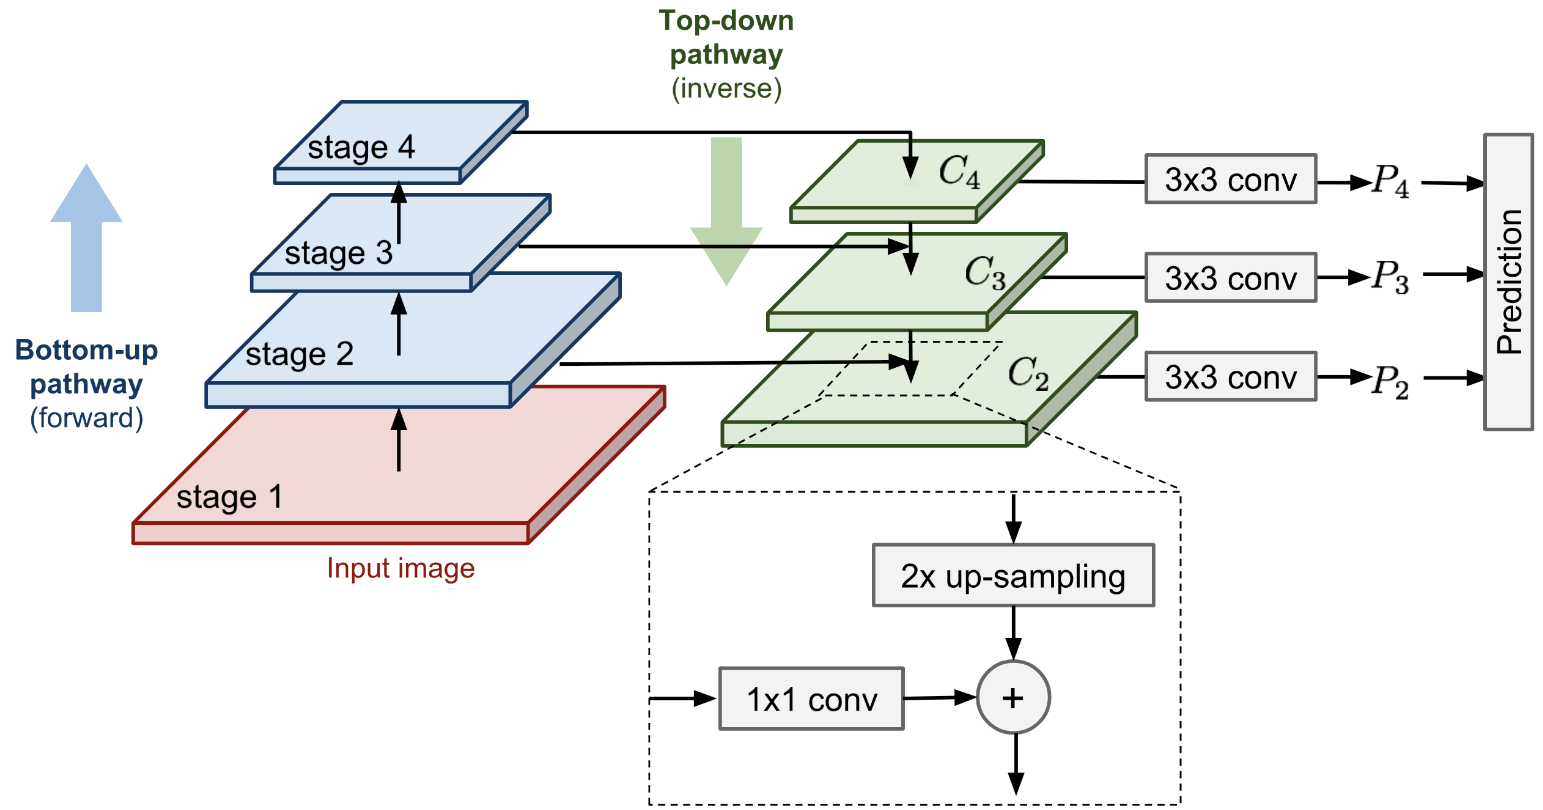
\includegraphics[width=0.4\linewidth]{./img/pyramid_network.png}
                    % \caption{Feature pyramid network workflow}
                \end{figure}
            \end{descriptionlist}

        \begin{remark}
            YOLOv3 predicts feature maps at scales 13, 26 and 52 using a feature pyramid network.
        \end{remark}

        \begin{figure}[H]
            \centering
            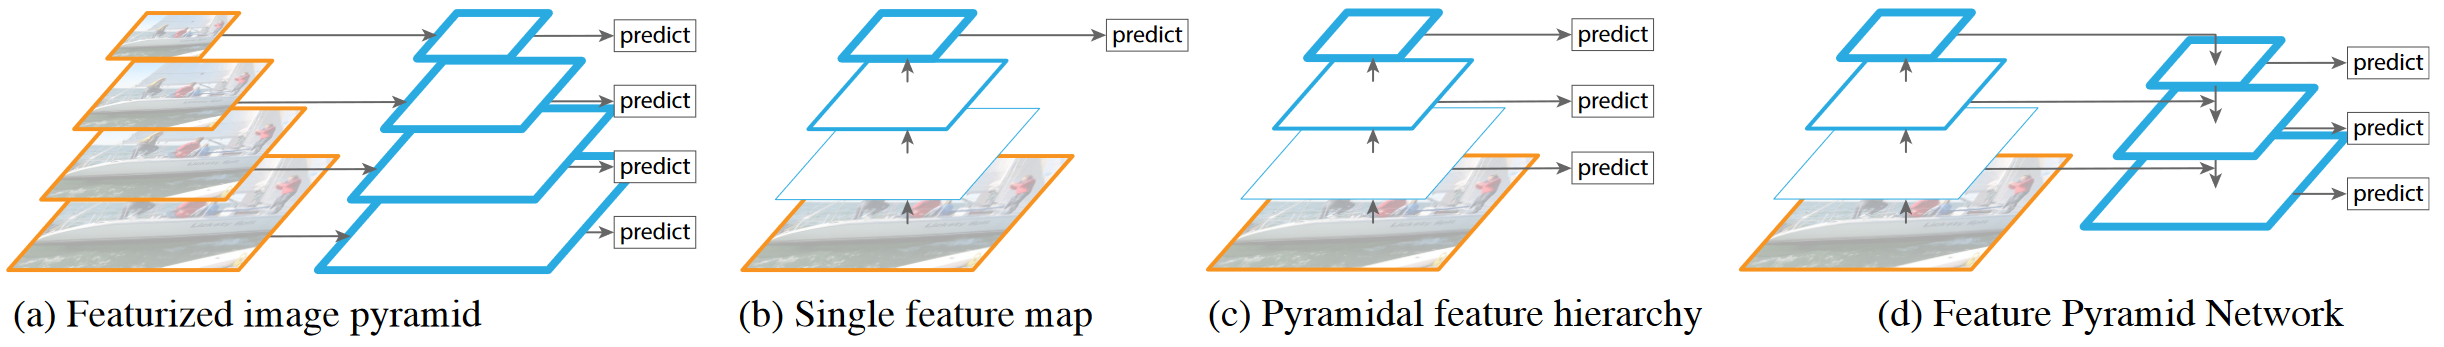
\includegraphics[width=0.95\linewidth]{./img/feature_pyramid.png}
            \caption{Feature pyramid recap}
        \end{figure}
\end{description}


\subsection{Non-maximum suppression}

\begin{description}
    \item[Non-maximum suppression] \marginnote{Non-maximum suppression}
        Method to remove multiple detections of the same object.

        Given the bounding boxes $BB_c$ of a class $c$ and a threshold $t$, NMS does the following:
        \begin{enumerate}
            \item Sort $BB_c$ according to the objectness score.
            \item While $BB_c$ is not empty:
            \begin{enumerate}
                \item Pop the first box $p$ from $BB_c$.
                \item $p$ is considered as a true prediction.
                \item Remove from $BB_c$ all the boxes $s$ with $\texttt{IoU}(p, s) > t$.
            \end{enumerate}
        \end{enumerate}
\end{description}